\chapter{IPv4}
\label{chap:ipv4}

\section{Ejercicio 1.1}

\subsection{Muestra una captura del tráfico de paquetes DHCP intercambiados entre el nodo host[0] y los servidores
DHCP durante el proceso de obtención de su IP, obtenida en Wireshark (Nota: para que los tiempos mostrados
en Wireshark coincidan con los tiempos de simulación, activa Visualización → Formato de visualización de fecha
→ Segundos desde 1970-01-01). Explica lo que ocurre y para qué sirve cada paquete. Para facilitar la captura,
configura el startTime del cliente DHCP para que se inicie antes en host[0] que el resto de equipos.}

\begin{figure}[H]
    \centering
    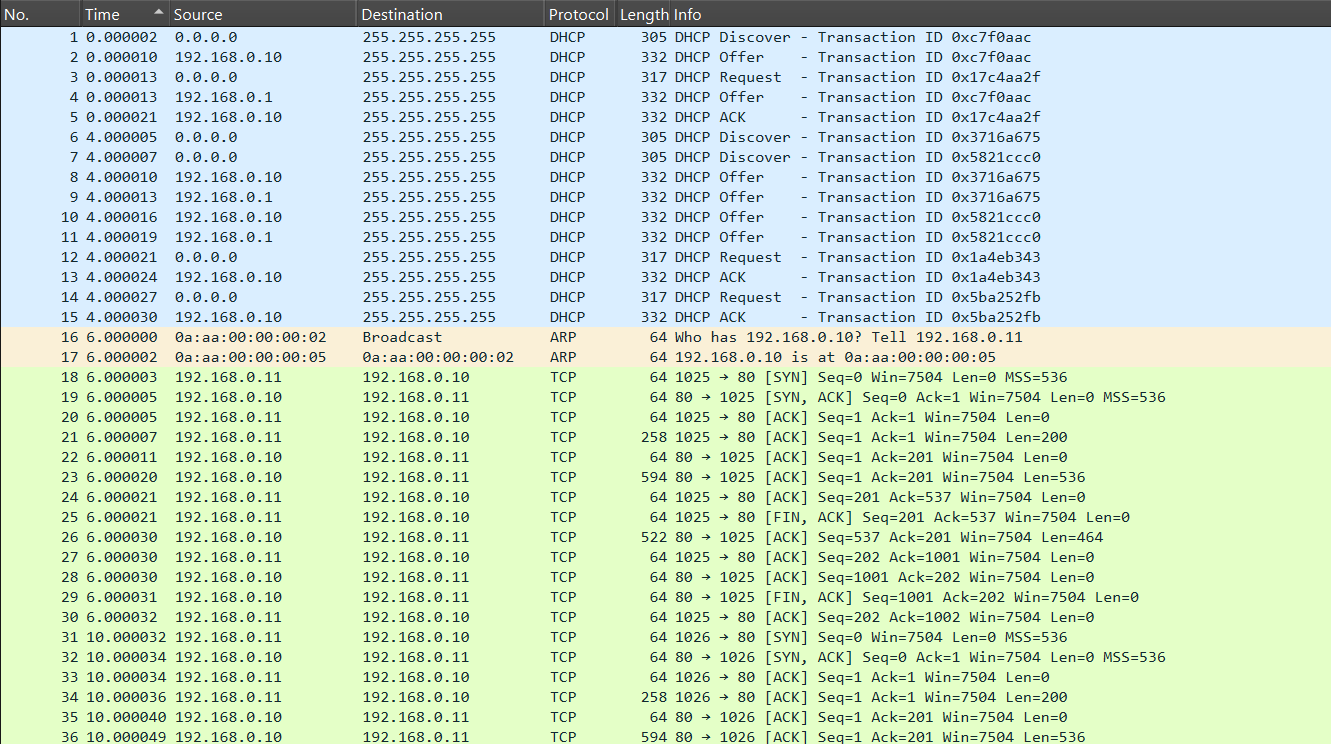
\includegraphics[width=135mm, scale=0.75]{imaxes/captura_ejer1_1.png}
    \caption{Tráfico DHCP entre host[0] y los servidores}
    \label{fig:captura_host0}
\end{figure}

Como podemos observar, el host[0] empieza enviando un DHCPDISCOVER con el objetivo de descubrir un servidor DHCP disponible. 
El servidor local resulta ser el primero en responder la solicitud con un paquete DHCPOFFER con una dirección IP disponible. El cliente (host[0]),
responde confirmando la elección del servidor local como su servidor DHCP y pidiendo la IP ofrecida mediante un DHCPREQUEST. El router también envía el paquete DHCPOFFER, pero lo hace más tarde, por lo que el cliente lo ignora y el router cancela la oferta (Ver \ref{sec:ej12}). Finalmente, el servidor local contesta con un DHCPACK confirmando la recepción del DHCPREQUEST y asignando definitivamente la IP elegida (Este proceso se repiten para los clientes host[1] y host[2]).

Posteriormente, el cliente host[0] intenta establecer una conexión con el servidor local, ya que este también ha sido configurado con una TcpGenericServerApp. Para ello, el cliente manda primero un broadcast ARP para averiguar cuál es la MAC de la máquina servidor con la IP que establece en la cabecera ARP. Después, el servidor contesta al broadcast ARP que mandó el cliente identificándose su MAC.

Finalmente, la conexión sigue adelante con los mensajes TCP correspondientes y repitiéndose cada 4 segundos (Esto ocurre ya que establecemos un idleInterval de 4 segundos).
\newline
\newline
Tipos de paquetes:
\begin{enumerate}
    \item DHCPDISCOVER: Para decubrir servidores DHCP disponibles. El cliente (en este caso host[0]) manda un paquete con IP destino de broadcast.
    \item DHCPOFFER: Respuesta del servidor a un paquete DHCPDISCOVER ofreciéndose como servidor DHCP. El servidor enviará un paquete donde la IP de origen será la del propio servidor (192.168.0.10) al destino 255.255.255.255, indicando además una IP ofrecida.
    \item DHCPREQUEST: El cliente confirma la elección de su servidor DHCP y le solicita la IP ofrecida. Esta comunicación sigue siendo broadcast para informar al resto de servidores DHCP, si los hubiere para que cancelen sus ofertas.
    \item DHCPACK: El servidor confirma la recepción de la petición por el cliente y le establece la IP solicitada. Este paquete tiene como destino la dirección de broadcast porque el cliente no ha recibido aún la IP, aunque se sabe a quién va dirigido gracias a un campo que incluye la MAC del cliente destino.
\end{enumerate}

\newpage

\section{Ejercicio 1.2}
\label{sec:ej12}
\subsection{¿Cuál de los servidores proporciona la IP a host[0]? ¿Sabe el otro servidor que host[0] no cogió la IP ofrecida por él? ¿Cómo? (Muestra el contenido de los paquetes relevantes en Wireshark.)}

Por lo que se puede ver en la figura \ref{fig:captura_host0}, en el intercambio inicial de paquetes DHCP, es el servidor local, con IP 192.168.0.10, quien envía el primer paquete DHCPOFFER. De esta manera, el servidor local, se adelanta al router, que envía su DHCPOFFER ya después de que el cliente responda con el DHCPREQUEST. Por tanto, es obvio deducir que el cliente está respondiendo y tomando la ip del servidor local. De todas formas, se pueden observar en detalle los paquetes 3 (DHCPREQUEST) y 5 (DHCPACK) para confirmar nuestra hipótesis. El paquete número 3 incluye los campos Requested IP Adress con la dirección IP solicitada por el cliente y DHCP Server Identifier con el servidor elegido para que le asigne esa IP. De igual forma, en el paquete número 5, aparece la IP asignada en el campo Your (client) IP Adress y el servidor que la asigna, de nuevo en la opción DHCP Server Identifier.
El router, que es el otro servidor DHCP, sí descubre que host[0] no coge su dirección IP, abandonando su oferta y dejando libre esa dirección para más adelante. Esto es gracias a que el paquete DHCPREQUEST, en el que el cliente contesta con la IP solicitada y el servidor al que se solicita, se envía a todos los posibles destinatarios dentro de la red 192.168.0.0.

\begin{figure}[H]
    \centering
    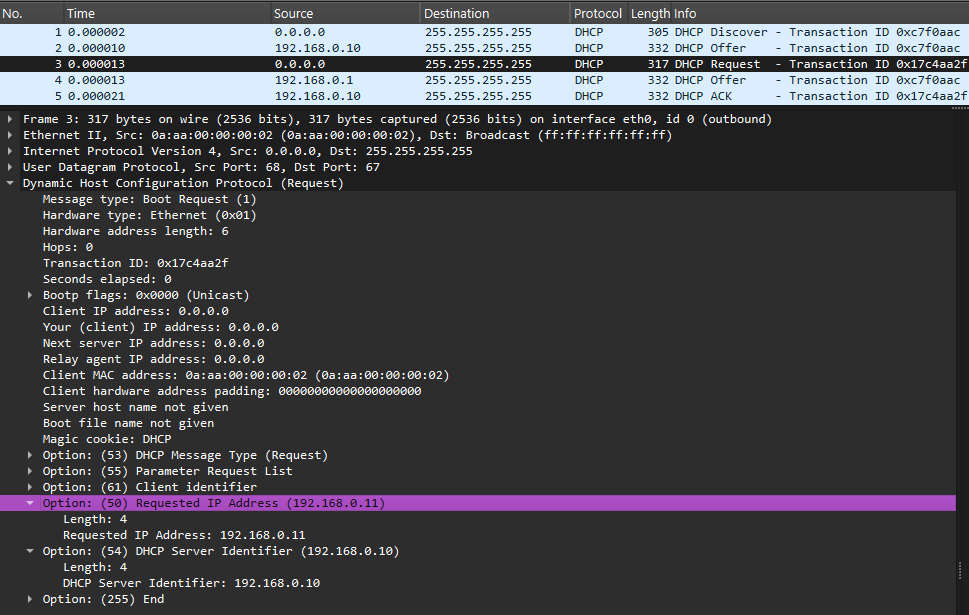
\includegraphics[width=135mm, scale=0.75]{imaxes/ejercicio1_3_1.png}
    \caption{Detalle de paquete DHCPREQUEST de host[0]}
    \label{fig:DHCPREQUEST_host0}
\end{figure}
\begin{figure}[H]
    \centering
    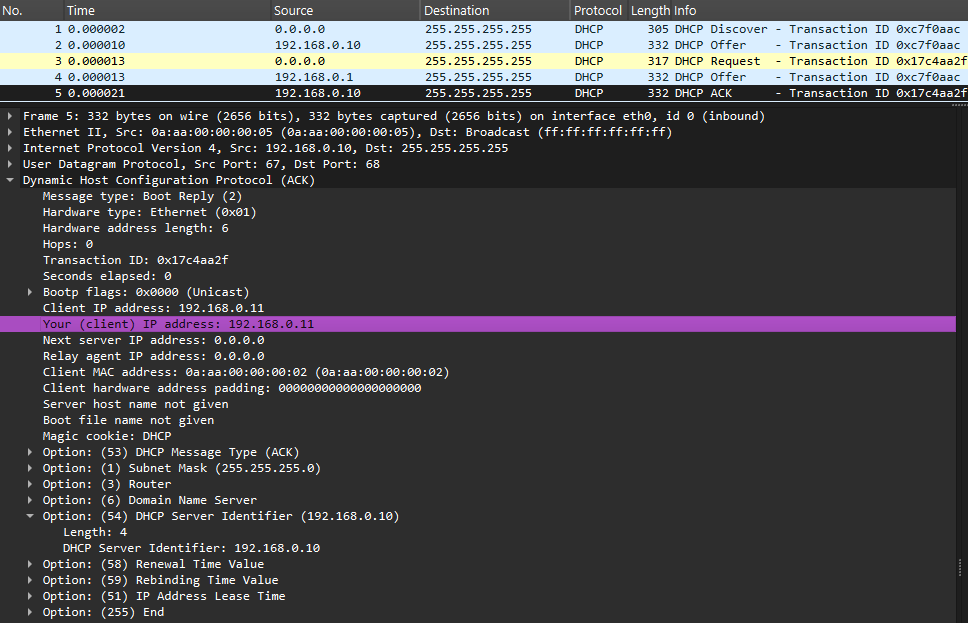
\includegraphics[width=135mm, scale=0.75]{imaxes/ejercicio1_3_2.png}
    \caption{Detalle de paquete DHCPACK de server\_local}
    \label{fig:DHCPACK_host0}
\end{figure}

\section{Ejercicio 1.3}

\subsection{¿De qué tipo son los primeros paquetes que se intercambian a partir de t = 6 segundos? ¿Cuál es su objetivo?}

Los primeros paquetes que se intercambian a partir de 6s son paquetes ARP. El objetivo de estos paquetes es mapear una dirección IP con su correspondiente dirección MAC. Depués, se guarda esta información en la caché ARP de los dispositivos involucrados. El host[0] pregunta por la MAC de la máquina con la IP 192.168.0.10, que es el servidor local que funciona como servidor TCP. Posteriormente, el servidor local responde enviando un paquete ARP de respuesta unicast al host con su dirección MAC. Sin este paso, no se podería establecer la conexión.

\section{Ejercicio 1.4}

\subsection{¿Cuáles son las direcciones origen y destino de estos paquetes (solicitud y respuesta)? ¿Tienen IP origen o destino? ¿Por qué?}

En el paquete de solicitud, la dirección de origen es la MAC del cliente TCP host[0], mientras que la dirección de destino es ff:ff:ff:ff:ff:ff, es decir, la dirección de broadcast MAC, cualquier dispositivo en la LAN. En el paquete de respuesta, la dirección origen es la MAC de server\_local y la dirección de destino la MAC de host[0]. 
Como ARP es un protocolo de capa de enlace, se envía a nivel ethernet y, por tanto, su origen y destino son, como se menciona anteriormente direcciones MAC y no IP. Sin embargo, las direcciones IP origen y destino sí estan incluídas en el protocolo ARP, y por lo tanto en el paquete, dentro de los campos sender/target IP address, como se aprecia en la imagen.

\begin{figure}[H]
    \centering
    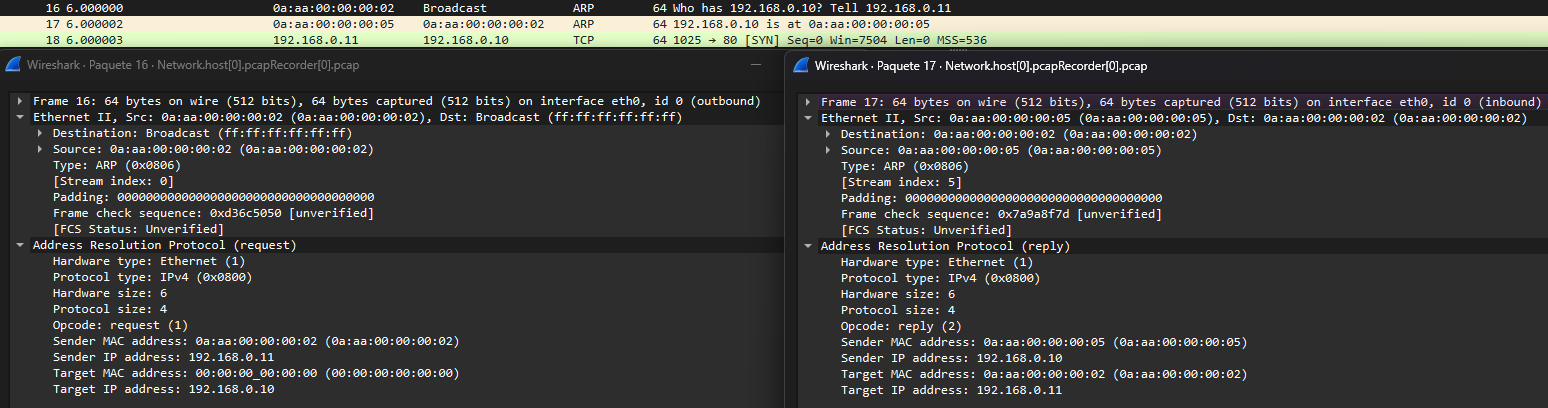
\includegraphics[width=135mm, scale=0.75]{imaxes/ejercicio1_4.png}
    \caption{Detalle del intercambio de paquetes ARP entre host[0] y server\_local}
    \label{fig:ARP_host0}
\end{figure}

\section{Ejercicio 1.5}

\subsection{Configura el servidor DHCP en serverlocal con numReservedAddresses = 10 y el cliente DHCP en host[2]
para que arranque antes que los otros clientes DHCP. Esto hará que host[2] reciba la IP fija asignada a
serverlocal (192.168.0.10). ¿Ocurre algún error cuando el host[2] recibe la IP de serverlocal? Configura el
cliente TCP en host[0] para que se conecte a serverlocal y describe paso a paso qué ocurre durante el
establecimiento de conexión TCP a partir de t = 6 segundos debido a esta duplicidad.}

Configurando la red para que el host[2] reciba de primero la IP con un numReservedAddresses = 10, efectivamente recibe la IP estática del servidor local tal y como lo menciona en el enunciado y no ocurre ningún error aunque tengamos dos dispositivos con la misma IP. No obstante, aunque no ocurra ningún error, esto puede desencadenar problemas en la red ya que habería un confrito de IPs como por ejemplo problemas de rendimiento en la red (retrasos en el procesamiento de paquetería o aumento de tráfico ARP al no poder resolver la MAC del disposivo),  pérdida de conexión, inconsistencias en las tablas ARP, etc.

\begin{figure}[!ht]
    \centering
    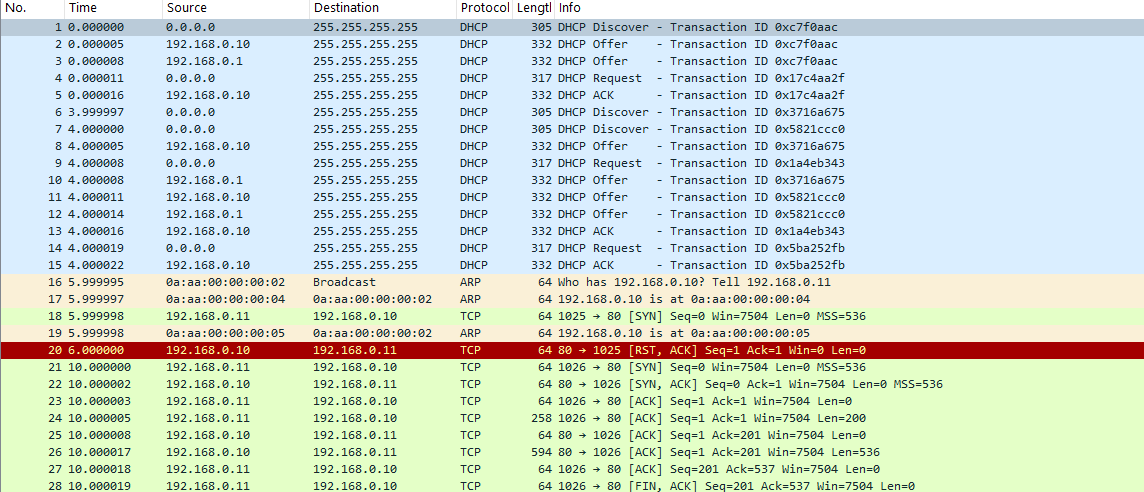
\includegraphics[width=135mm, scale=0.75]{imaxes/captura_ejer1_5.png}
    \caption{Tráfico DHCP entre host[0] y los servidores cuando host[2] recibe la ip servidor local}
    \label{fig:captura2_host0}
\end{figure}

Configurando el cliente TCP en el host[0], como se puede ver en la imagen \ref{fig:captura2_host0}, el host[0] manda un paquete ARP modo broadcast para averiguar la MAC del dispositivo con la ip 192.168.0.10. Le contesta primero el servidor local, por lo que empieza la conexión en capa 4; pero, poco después, el host[2] contesta también al broadcast mandado por el host[0], ya que él tiene la misma IP asignada que el servidor local, por lo que se interrumpe la conexión del host[0] con el servidor local mandando un RST,ACK. Pasados 4 segundos (ya que establecemos un idleInterval de 4 segundos), se vuelve establecer la conexión entre host[0] y el server local haciendose esta de manera exitosa ya que en la tabla ARP del host[0] se almacenó como dispositivo correspondiente a la IP 192.168.0.10, la MAC de servidor local ya que fue el primer dispositivo en responde al mandar paquetes ARP en modo broadcast .
